% Questions on PDF page 134
\documentclass[11pt]{article}

\usepackage[utf8]{inputenc}
\usepackage[a4paper, margin=1in]{geometry}
\usepackage{booktabs}
\usepackage{enumerate}
\usepackage{physics}
\usepackage{amsmath}
\usepackage{amsfonts}
\usepackage{graphicx}
\usepackage{siunitx}
\usepackage{textcomp}
\usepackage{hyperref}

\bibliographystyle{ieeetr}
\graphicspath{{./figures}}

\title{Big Data (AES 630) Homework 3}
\author{Mitchell Dodson}
\date{February 22, 2024}

\newcommand*{\problem}[2]{
    \begin{table}[ht]
    \centering
        \begin{tabular}{ | p{.1\linewidth} p{.9\linewidth} | }
            \hline
            \vspace{.3em}\textbf{\large#1:} & \vspace{.3em}\small{#2}\hspace{.2em}\vspace{.5em} \\ \hline
        \end{tabular}
    \end{table}
}

\begin{document}

\noindent
{\Large\textbf{Big Data (AES 690) Homework 3}}

\noindent
\large{Mitchell Dodson}

\noindent
\large{February 22, 2024}

\vspace{1em}
\noindent
{\Large\textbf{Predictor trained on Alabama ASOS data}}

\begin{figure}[h!]
    \centering

    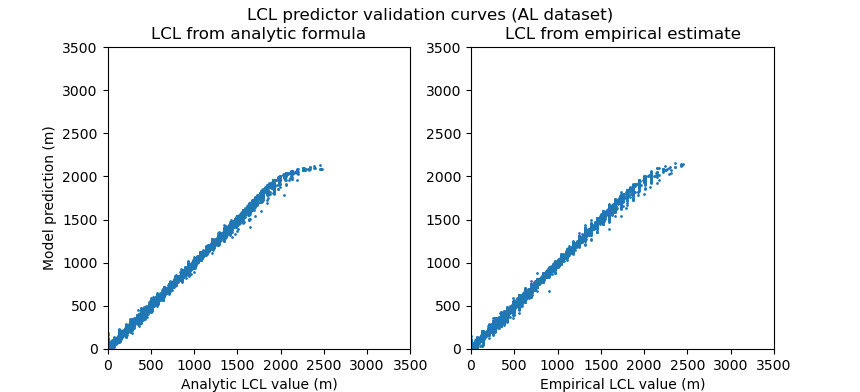
\includegraphics[width=.6\paperwidth]{figs/val_ff-rand-014_al.png}

    \caption{Feedforward network validation curves for emulating analytic LCL calculations (left) and empirical LCL estimates (right). Data used for evaluation includes training and validation data from Alabama ASOS stations in July, 2023. $R^2=99.82\%$ for the analytic predictions and $R^2=99.81\%$ for the empirical predictions. Mean absolute error magnitudes were $14.23\,\si{m}$ and $14.32\,\si{m}$, respectively.}
    \label{f1}
\end{figure}

Figure \ref{f1} shows the validation curves of a 7-layer feed-forward predictor with 14,002 parameters. The model receives surface measurements of the temperature, relative humidity, wind speed, and mean pressure as inputs, then generates predictions for the LCL height in meters as calculated by the formula from (Romps, 2017), and an empirical estimate, respectively. In both cases, the predictions generally trend well, but start to underestimate the LCL height in the upper extremes of values represented by the dataset. This may be caused by bias in the training sample distribution, which over-represents surface conditions near saturation (and subsequently having lower LCL heights).

\begin{figure}[h!]
    \centering

    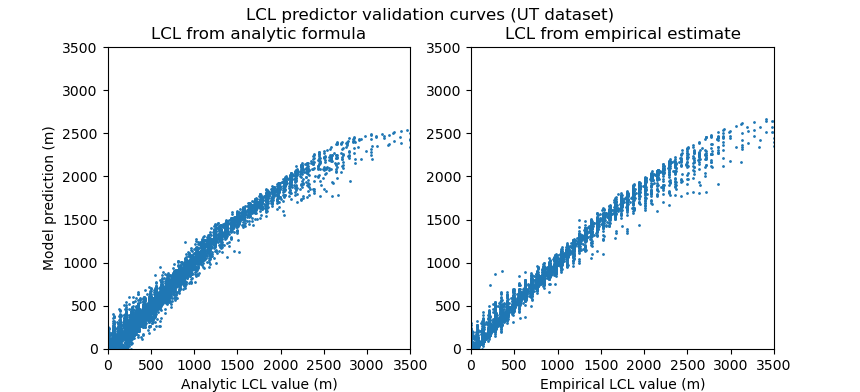
\includegraphics[width=.6\paperwidth]{figs/val_ff-rand-014_ut.png}

    \caption{Validation curves for the same model as above, evaluated on unseen ASOS data from Utah in March 2023. $R^2=96.64\%$ for the analytic predictions and $R^2=97.21\%$ for the empirical predictions. Mean absolute errors were $67.1\,\si{m}$ and $55.1\,\si{m}$, respectively.}
    \label{f2}
\end{figure}

\newpage

As the point distributions in Figure \ref{f2} indicate, the same model struggled to generalize to the more arid conditions from the March 2023 ASOS data from Utah stations. Due to the dry conditions, the unseen dataset contains much higher LCL heights than did the data used to train the model. As such, the highest LCL heights predicted by the model are only about $2,500\,\si{m}$ (the upper limit of training data), while the corresponding actual values reach heights of more than $3,000\,\si{m}$. Even LCL values within the normal range of the training data have prediction error magnitude around four times higher than that of Alabama stations.

\begin{figure}[h!]\label{q1q2}
    \centering
    \begin{tabular}{ c c c | c}
    \end{tabular}
\end{figure}

\vspace{-1em}
\noindent
{\Large\textbf{Predictor trained on combined ASOS data}}


\begin{figure}[h!]
    \centering

    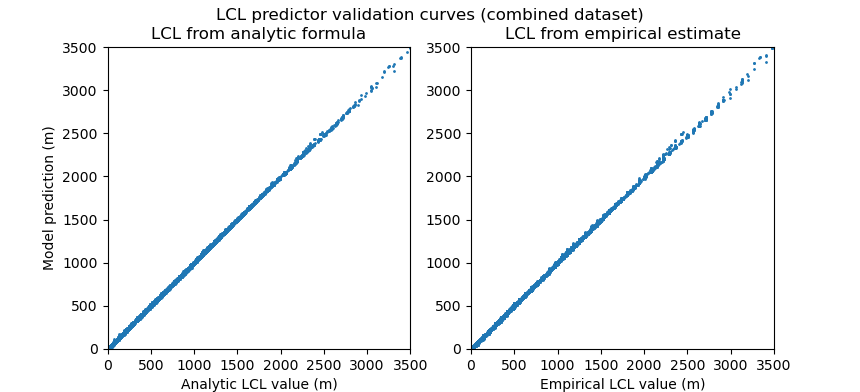
\includegraphics[width=.6\paperwidth]{figs/val_ff-combined-01_combined.png}

    \caption{Validation curves for a feedforward model trained on ASOS data from Alabama as well as Utah, evaluated on its training and validation data. $R^2=99.983\%$ for the analytic predictions and $R^2=99.973\%$ for the empirical predictions. Mean absolute errors were $5.46\,\si{m}$ and $6.77\,\si{m}$, respectively.}
    \label{f3}
\end{figure}

The next model is an 11-layer feedforward model with 164,050 parameters, trained on the same four input variables including data from both Alabama and Utah. After training on only 60\% of the data (the other 40\% going towards validation), the new model achieved considerably lower error rates than previous iterations when evaluated on the full dataset. Although it isn't surprising that a much larger model would make a better prediction, the 14,002 parameter model from the first section outperformed much larger models trained on the same data. With this in mind, I suspect that fitting the model on the additional data  reduced the bias of the training set, and enabled the model to discover more general representation of the relationship between surface conditions and LCL altitude.

It's worth noting that the model architectures used in this report were selected by randomly searching plausible hyperparameter configurations forming a solution space with size 207,360. The hyperparameters subject to variation include model type, layer and node count, learning rate, feature masking amount, activation function, and dropout rates. With a sample size of 128 models, the most performant had at least 6 layers, a wide variety of layer widths, no dropout, no masking, logistic activation functions, and learning rate ceilings between \num{1e-4} and \num{1e-6}.

\vspace{1em}
\centering\large
\textbf{My code for this assignment is available on github at:}

\centering\large
\url{https://github.com/Mitchell-D/aes690hw3}

\vspace{.5em}

\centering\large
\textbf{Models were developed with the tracktrain workflow:}

\centering\large
\url{https://github.com/Mitchell-D/tracktrain}

\end{document}

\begin{figure}[h!]\label{q1q2}
    \centering
    \begin{tabular}{ c c c | c}
    \end{tabular}
\end{figure}

